\chapter{Geometrische simpliziale Komplexe}
\section{Definition und erste Eigenschaften} % TODO: besserer Name?
Oftmals ist es hilfreich, einen topologischen Raum in kleinere Bausteine zu
unterteilen. Eine typische solche Unterteilungsmöglichkeit sind \emph{CW-Komplexe}, welche
aber für kombinatorische Anwendungen noch zu allgemein sind.\footnote{%
    In der Tat kann man zeigen, dass es CW-Komplexe gibt, welche sich nicht
    durch die nachfolgenden Konstruktionen beschreiben lassen. Dass dies sogar
    schon mit einem zweidimensionalen CW-Komplex möglich ist, zeigt
    beispielsweise Bognár\cite{artcle:bognar77}. Ein Beispiel für einen
    dreidimensionalen solchen CW-Komplex findet man bei
    Lundell\cite[Ch.\,III,\;1.8]{bookc:lundell69}.%
}
Wir interessieren uns daher dafür, wie wir topologische Räume beschreiben
können, die aus kombinatorisch einfacher zu beschreibenden Bausteinen aufgebaut
sind. Namentlich werden dies \emph{Punkte, Strecken, Dreiecke, Tetraeder} und
höherdimensionale Objekte desselben Typus sein, welche mathematisch durch
sogenannte \emph{Simplizes} beschrieben werden können. Dazu benötigen wir
zunächst die folgenden Begriffe:

\begin{thDef}[Affin (un-)abhängig]
    Sind $n,d\in\N$ und $v_0,\ldots,v_n\in\R^d$, so bezeichnen wir diese
    Vektoren als \emph{affin abhängig}, falls es Elemente
    $\lambda_0,\ldots,\lambda_n \in\R$ mit folgenden drei Eigenschaften gibt:
    \[ \{\lambda_0,\ldots,\lambda_n\} \neq \{0\}, \quad \isum^n \lambda_i = 0
    \qundq \isum^n \lambda_i\,v_i = 0 \in\R^d.\] 
    Falls es solche Zahlen nicht gibt, so bezeichnen wir die Vektoren als
    \emph{affin unabhängig}.
\end{thDef}

\begin{thLemma}[Äquivalente Bedingung für affine Unabhängigkeit]
    \label{gsc:iffaffinlyindependet}
    %
    Seien $n,d\in\N$. Dann sind $v_0,\ldots,v_n\in\R^d$ genau dann affin
    unabhängig, wenn ein $k\in\setZeroto{n}$ existiert, so dass die Familie
    \[  (v_i - v_k)_{i \in\setZeroto{n}\setminus\{k\}} \] 
    von Vektoren im $\R^d$ linear unabhängig ist.
\end{thLemma}

Der Beweis ist eine einfache Übung.
Aus \cref{gsc:iffaffinlyindependet} folgt insbesondere, dass für $d\in\N$
maximal $d+1$ Vektoren im $\R^d$ affin unabhängig sein können.

\begin{thDef}[Konvexe Menge, konvexe Hülle, Konvexkombination]
    Sei $d\in\N$. Eine Teilmenge $A\subset\R^d$ heißt \emph{konvex}, wenn
    für alle $x,y\in A$ auch die (lineare) Verbindungsstrecke
    \[ \{ tx + (1-t)\,y \Mid t\in[0,1] \} \]
    in~$A$ enthalten ist.

    \newpage
    \noindent
    Für eine Teilmenge $A'\subset\R^d$ definiert
    \[ \conv(A') \defeq 
        \bigcap \,\bigl\{ A\subset\R^d \Mid A'\subset A\text{ konvex} \bigr\}
    \]
    die \emph{konvexe Hülle von $A'$}.
    %
    Sind außerdem $n\in\N$ und $v_0,\ldots,v_n\in\R^d$ sowie
    $\lambda_0,\ldots,\lambda_n\in\R[\geq0]$ mit $\isum^n\lambda_i = 1$, so
    bezeichnet man $\isum^n \lambda_i\,v_i$ als eine \emph{Konvexkombination der
    $v_i$}.
\end{thDef}

\begin{thBemerkung} \label{gsc:convexhullviaconvexcombinations}
    Mithilfe einfacher Argumente zeigt man außerdem, dass für eine Teilmenge
    $A'\subset\R^d$ die konvexe Hülle $\conv(A')$ gerade aus allen 
    Konvexkombinationen je endlich vieler Elemente aus $A'$ besteht.
\end{thBemerkung}


\begin{thDef}[(Geometrisches) Simplex, Eckpunkte, Dimension]
    \label{gsc:def:simplex}
    %
    Ist $d\in\N$ und $A\subset\R^d$ eine endliche Menge affin unabhängiger
    Vektoren im $\R^d$ (oder leer), so bezeichnet man $\sigma \defeq \conv(A)$ als
    \emph{(geometrisches) Simplex} und nennt die Elemente aus $A$
    \emph{Eckpunkte (von~$\sigma$)}, oder kurz \emph{Ecken (von~$\sigma$)}. Die
    \emph{Dimension von $\sigma$} ist dann durch $\dim(\sigma) \defeq \abs{A}-1$
    definiert (-- mittels \cref{gsc:iffaffinlyindependet} zeigt man leicht, dass
    dies wohldefiniert ist --) und man nennt ein $n$-dimensionales Simplex auch
    kurz \emph{$n$-Simplex} (wobei $n\in\N\cup\{-1\}$).
    (Siehe \cref{gsc:fig:simplices})
\end{thDef}

\begin{thDef}[Seite eines Simplex]
    Ist $d\in\N$ und $\sigma$ ein Simplex mit der Eckenmenge $E \subset\R^d$, so
    ist die konvexe Hülle $\conv(E')$ einer Teilmenge $E'$ von $E$ wieder ein
    Simplex und jedes dieser Simplizes wird als \emph{Seite von $\sigma$}
    bezeichnet.
\end{thDef}
\unskip  % FIXME: Why is this needed here!?

\begin{figure}
    \centering
    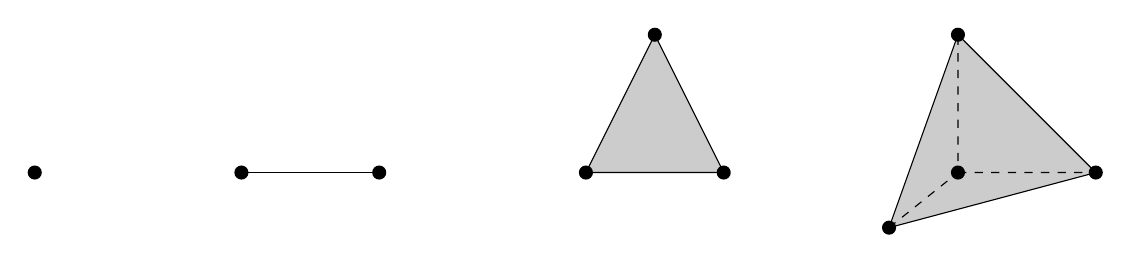
\begin{tikzpicture}[%
            scale=1.75,
            mypoint/.style={shape=circle, inner sep=1.8pt, color=black, fill}
        ]
        \begin{scope}
            \node at (0,0) [mypoint] {};
        \end{scope}
        \begin{scope}[shift={(1.5,0)}]
            \draw (0,0) node [mypoint] {} -- (1,0) node [mypoint] {};
        \end{scope}
        \begin{scope}[shift={(4,0)}]
            \draw [fill=black!20] (0,0) node [mypoint] {} -- 
                  (1,0) node [mypoint] {} --
                  (0.5,1) node [mypoint] {} -- cycle ;
        \end{scope}
        \begin{scope}[shift={(6.7,0)},z={(-5mm,-4mm)}]
            \coordinate (A) at (0,0,1);
            \coordinate (B) at (1,0,0);
            \coordinate (C) at (0,1,0);
            \coordinate (D) at (0,0,0);
            
            \draw [fill=black!20]
                  (A) node [mypoint] {} --
                  (B) node [mypoint] {} --
                  (C) node [mypoint] {} -- cycle
                  (D) node [mypoint] {};
            \draw [dashed] (A) -- (D) -- (C) (D) -- (B);
        \end{scope}
    \end{tikzpicture}
    \caption{$0$- bis $3$-dimensionale Simplizes}
    \label{gsc:fig:simplices}
\end{figure}

\begin{thDef}%
    [Geometrischer simplizialer Komplex, Dimension, Polyeder, Eckenmenge]
    \label{gsc:def:gsc}
    %
    Sei $d\in\N$. Ist $\Delta$ eine nicht-leere Menge von (geometrischen)
    Simplizes im $\R^d$, so ist $\Delta$ ein \emph{(geometrischer) simplizialer
    Komplex}, falls folgende Bedingungen erfüllt sind:
    \begin{itemize}
        \item Ist $\sigma$ ein Simplex in $\Delta$, so ist auch jede Seite von
            $\sigma$ in $\Delta$ enthalten.
        \item
            Der Schnitt zweier Simplizes $\sigma_1,\sigma_2\in\Delta$ ist eine
            Seite von $\sigma_1$ und $\sigma_2$.
    \end{itemize}
    Wir definieren die \emph{Dimension von $\Delta$} als die maximale Dimension
    seiner Simplizies:
    \[ \dim(\Delta) \defeq \max\{ \dim(\sigma) \Mid \sigma\in\Delta \} \;\in\N
    . \]
    Ist $\Delta$ ein simplizialer Komplex, so setzen wir
    \[ \polyeder\Delta \defeq \bigcup \Delta \;\subset\R^d \]
    und statten diesen Raum mit der von den Inklusionen der einzelnen Simplizes
    induzierten Finaltopologie aus. Explizit bedeutet das hier:
    $A\subset\polyeder\Delta$ ist genau dann offen (abgeschlossen), wenn für alle
    $\sigma\in\Delta$ der Schnitt $A\cap\sigma$ offen (abgeschlossen) in
    $\sigma$ ist (wobei $\sigma$ die Teilraumtopologie trägt). Wir nennen dann
    $\polyeder\Delta$ das \emph{zu $\Delta$ gehörige Polyeder}.
    Außerdem definieren wir $V(\Delta)$ als die Vereinigung
    aller Eckenmengen von Simplizes in $\Delta$.
    (Siehe \cref{gsc:fig:simplicialcomplex}.)
\end{thDef}

\Achtung
In der Literatur wird des Öfteren der Fall des leeren Simplex~$\emptyset$
ausgeschlossen. Nach den obigen Definitionen \ref{gsc:def:simplex} und 
\ref{gsc:def:gsc} ist dies aber erlaubt und insbesondere enthält jeder
simpliziale Komplex das leere Simplex.

\begin{figure}
    \centering
    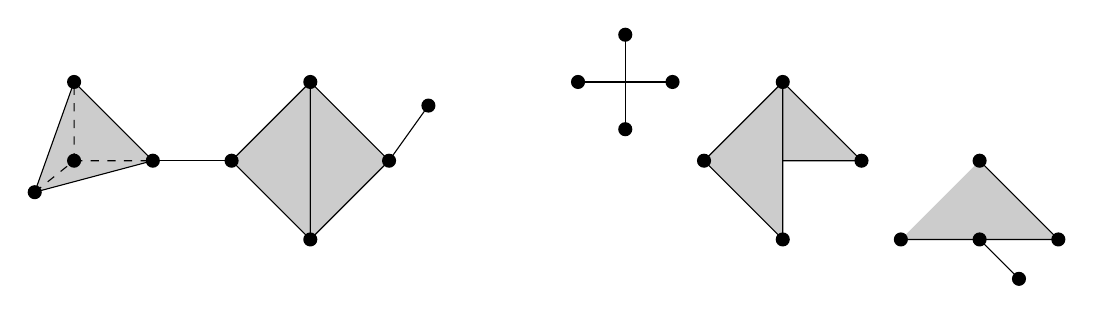
\begin{tikzpicture}[%
            mypoint/.style={shape=circle, inner sep=1.8pt, color=black, fill}
        ]
        \begin{scope}[z={(-5mm,-4mm)}]
            \coordinate (A) at (0,0,1);
            \coordinate (B) at (1,0,0);
            \coordinate (C) at (0,1,0);
            \coordinate (D) at (0,0,0);
            
            \coordinate (E) at (2,0,0);
            \coordinate (F1) at (3,1,0);
            \coordinate (F2) at (3,-1,0);
            \coordinate (G) at (4,0,0);
            \coordinate (H) at (4.5,0.7,0);
            
            \draw [fill=black!20]
                  (A) node [mypoint] {} --
                  (B) node [mypoint] {} --
                  (C) node [mypoint] {} -- cycle
                  (D) node [mypoint] {};
            \draw [dashed] (A) -- (D) -- (C) (D) -- (B);
            
            \draw (B) -- (E);
            \draw [fill=black!20] (E) -- (F1) -- (F2) -- cycle;
            \draw [fill=black!20] (G) -- (F1) -- (F2) -- cycle;
            \path (E)  node [mypoint] {} 
                  (F1) node [mypoint] {}
                  (F2) node [mypoint] {};
            
            \draw (G) node [mypoint] {} -- (H) node [mypoint] {};
        \end{scope}
        
        \begin{scope}[shift={(7,1)},scale=0.6]
            \draw (-1,0) node [mypoint] {} -- (1,0) node [mypoint] {}
                  (0,-1) node [mypoint] {} -- (0,1) node [mypoint] {};
        \end{scope}
        
        \begin{scope}[shift={(6,0)}]
            \coordinate (E) at (2,0,0);
            \coordinate (F1) at (3,1,0);
            \coordinate (F2) at (3,-1,0);
            \coordinate (F3) at (3,0,0);
            \coordinate (G) at (4,0,0);
            
            \draw [fill=black!20] (E) -- (F1) -- (F2) -- cycle;
            \draw [fill=black!20] (G) -- (F1) -- (F3) -- cycle;
            \path (E)  node [mypoint] {} 
                  (F1) node [mypoint] {}
                  (F2) node [mypoint] {}
                  (G)  node [mypoint] {};
        \end{scope}
        
        \begin{scope}[shift={(10.5,-1)}]
            \draw [fill=black!20] 
                (0,0) node [mypoint] {} --
                (2,0) node [mypoint] {} -- 
                (1,1) node [mypoint] {};
            \draw (1,0) node [mypoint] {} -- (1.5,-0.5) node [mypoint] {};
        \end{scope}
    \end{tikzpicture}
    \caption{Simplizialer Komplex (links) und 
             \emph{keine} simplizialen Komplexe (rechts)}
    \label{gsc:fig:simplicialcomplex}
\end{figure}

\begin{thDef}[Rand und Inneres eines Simplex]
    Ist $\sigma$ ein Simplex, so bezeichnen wir die Vereinigung aller Seiten von
    $\sigma$ mit Dimension echt kleiner als $\dim(\sigma)$ als \emph{Rand von
    $\sigma$} und die Teilmenge von $\sigma$, die sich ergibt, wenn wir aus
    $\sigma$ den Rand entfernen, als \emph{(relatives) Inneres von $\sigma$}.
\end{thDef}

\begin{thDef}[Träger]
    Ist $\Delta$ ein simplizialer Komplex und $x\in\polyeder\Delta$, so kann man
    zeigen, dass es genau ein Simplex $\sigma\in\Delta$ gibt, für das $x$ im
    Inneren von $\sigma$ liegt. Dieses bezeichnen wir als \emph{Träger von~$x$}
    und schreiben dafür $\supp(x)$.
\end{thDef}

\begin{thDef}[Teilkomplex, \texorpdfstring{$k$}{k}-Skelett]
    Sei $\Delta$ ein simplizialer Komplex. Wir nennen $\Delta'\subset\Delta$
    einen \emph{Teilkomplex}, falls $\Delta'$ selbst einen simplizialen Komplex
    definiert.
    Für jedes $k\in\setZeroto{\dim(\Delta)}$ ist
    \[ \skeleton\Delta{k} 
        \defeq \bigl\{ \sigma\in\Delta \Mid \dim(\sigma)\leq k \bigr\}
    \]
    ein Teilkomplex von $\Delta$, welchen wir \emph{$k$-Skelett von $\Delta$}
    nennen. (Insbesondere gilt für $k=0$: $\skeleton\Delta0 = V(\Delta)$.)
\end{thDef}

\medskip
Im Folgenden werden wir hauptsächlich \emph{endliche} simpliziale Komplexe
betrachten, d.\,h. simpliziale Komplexe mit nur endlich vielen Simplizes. Daher
halten wir noch folgende Aussage fest:

\begin{thLemma}[Polyeder eines endlichen simplizialen Komplexes]
    Ist $d\in\N$ und $\Delta$ ein endlicher simplizialer Komplex im $\R^d$, 
    so stimmt die Topologie auf $\polyeder\Delta$ aus \cref{gsc:def:gsc} mit 
    der Teilraumtopologie von $\polyeder\Delta$ als Teilmenge des $\R^d$
    überein.
\end{thLemma}

Der Beweis ist einfach und wird an dieser Stelle dem Leser zur Übung überlassen.
(Siehe beispielsweise Munkres\cite[Ch.\,1,\;\S2]{bookc:munkres84}.)

Einfache aber nützliche Beispiele für endliche simpliziale Komplexe liefert das
folgende Lemma:

\begin{thLemma}[Simplizialer Komplex eines Simplex]
    \label{gsc:complexofsimplex}
    %
    Sind $n,d\in\N$ und ist $\sigma$ ein $n$-Simplex im $\R^d$, so ist
    \[ \Delta(\sigma) 
        \defeq \{ \sigma' \Mid \sigma' \text{ ist Seite von } \sigma \}
    \]
    ein $n$-dimensionaler (endlicher) simplizialer Komplex im $\R^d$.
\end{thLemma}

\begin{proofsketch}
    Falls $\Delta(\sigma)$ ein simplizialer Komplex ist, ist klar, dass dieser
    endlich ist, da die Anzahl der Ecken von $\sigma$ endlich ist. Außerdem gilt
    $\sigma\in\Delta(\sigma)$, womit $\dim\bigl(\Delta(\sigma)\bigr) = n$ klar
    ist. Es bleibt also zu zeigen, dass $\Delta(\sigma)$ einen simplizialen
    Komplex definiert. Die erste Bedingung in \cref{gsc:def:gsc} ist dabei
    offensichtlich erfüllt und für die zweite zeigt man mithilfe von
    \cref{gsc:convexhullviaconvexcombinations} und einfachen Umformungen, dass
    für Teilmengen $A,B$ der Eckenmenge von $\sigma$ stets $\conv(A)\cap\conv(B)
    = \conv(A\cap B)$ gilt.
    \\
\end{proofsketch}

Das letzte Argument findet man ausführlicher auch bei 
Matou\v sek\cite[Ch.\,1,\;1.3.6]{bookc:matousek03}.


\section{Triangulierung}
\begin{thDef}[Triangulierbar, Triangulierung]
    Ein topologischer Raum~$X$ heißt \emph{triangulierbar}, falls es
    einen simplizialen Komplex $\Delta$ und einen Homöomorphismus
    $\polyeder\Delta \cong X$ gibt. Solch einen Homöomorphismus nennen wir 
    eine \emph{Triangulierung von $X$}.
\end{thDef}

Die folgenden Aussagen liefern uns Triangulierungen für Sphären jeder
Dimension:

\begin{thLemma}[Kompaktheit konvexer Hülle endlich vieler Punkte]
    \label{gsc:convexhullcompact}
    %
    Ist $d\in\N$ und $A\subset\R^d$ eine endliche Teilmenge, so ist die konvexe
    Hülle $\conv(A)\subset\R^d$ eine kompakte Menge.
\end{thLemma}

\begin{proof}
    Seien $n\in\N$ und $v_0,\ldots,v_n$ die verschiedenen Punkte aus $A$
    (wobei o.\,E. $A\neq\emptyset$).
    Nach \cref{gsc:convexhullviaconvexcombinations} gilt dann:
    \[ \conv(\{v_0,\ldots,v_n\}) = 
        \Bigl\{\, \isum^n \lambda_i\,v_i \Mid[\;] \lambda\in(\R[\geq0])^{n+1},
        \; \isum^n \lambda_i = 1    \,\Bigr\}
    . \]
    Die Menge 
    $T\defeq\{ \lambda\in [0,1]^{n+1} \Mid \isum^n \lambda_i = 1 \}$
    ist abgeschlossen in $[0,1]^{n+1}$ als Urbild der in $\R$ abgeschlossenen
    Menge $\{1\}$ unter der stetigen Funktion $[0,1]^{n+1}\to\R,\;
    \lambda\mapsto\isum^n \lambda_i$. Weil $[0,1]^{n+1}$ kompakt ist, ist somit
    auch $T$ kompakt. Damit ist die obige konvexe Hülle kompakt als Bild der
    kompakten Menge~$T$ unter der stetigen Abbildung
    \[ T \to \R^d, \quad \lambda\mapsto \isum^n \lambda_i\,v_i \mkern2mu . \]
\end{proof}

\begin{thKorollar}[Simplizes sind kompakt]
    \label{gsc:simplicescompact}
    %
    Ist $\sigma$ ein Simplex, so ist $\sigma$ mit der Teilraumtopologie ein
    kompakter topologischer Raum.
\end{thKorollar}

\begin{thSatz}[Homöomorphie zwischen Bällen und konvexen Mengen]
    \label{gsc:convexsethomeodisk}
    %
    Sei $d\in\N$ und $A\subset\R^d$ eine konvexe und kompakte Teilmenge mit
    nicht-leerem Inneren $\setinterior A$. Dann gibt es einen Homöomorphismus
    \[ f\colon A \isorightarrow D^d \qqtextqq{mit} 
        f\vert_{\setboundary{A}}\colon \setboundary{A} \isorightarrow 
        S^{d-1} \subset D^d 
    . \]
\end{thSatz}

Einen Beweis dieses Satzes findet man beispielsweise bei
Bredon\cite[Ch.\,I,\;16.]{bookc:bredon93} oder bei
Munkres\cite[Ch.\,1,\;\S1,\;1.1]{bookc:munkres84}.

\begin{thBeispiel}\label{gsc:bsp:spheretriang}
    Zu $d\in\N[\geq1]$ erhalten wir also eine Triangulierung der Sphäre
    $S^{d-1}$ wie folgt: Sei $\sigma$ ein $d$-Simplex. Wir bilden
    dann den zugehörigen simplizialen Komplex und entfernen die einzige
    $d$-dimensionale Seite (also $\sigma$ selbst). Wir erhalten so einen
    simplizialen Komplex $\Delta(\sigma)\setminus\{\sigma\}$, dessen Polyeder
    nach \cref{gsc:simplicescompact} und \cref{gsc:convexsethomeodisk} zur
    Einheitssphäre~$S^{d-1}$ homöomorph ist. Ein Homöomorphismus ist dann
    gerade durch die Zentralprojektion von einem Punkt im Inneren des Simplex
    aus auf die Sphärenoberfläche gegeben (siehe \cref{gsc:fig:spheretriang}).
    Nehmen wir ohne Einschränkung an, dass $0$ im Inneren von
    $\polyeder{\Delta(\sigma)\setminus\{\sigma\}}$ liegt, dann ist eine
    entsprechende Zentralprojektion gerade durch die Abbildung
    \[ \polyeder{\Delta(\sigma)\setminus\{\sigma\}} \to S^{d-1},\quad
        x\mapsto \frac{x}{\norm{x}_{\mathrlap{2}}}
    \]
    gegeben, wobei $\norm{\,\cdot\,}_2$ die euklidsche Norm bezeichnet.
\end{thBeispiel}

\begin{figure}
    \centering
    \begin{tikzpicture}[scale=2.9]
        \draw (0,0) -- (1,0) -- ++(120:1) -- cycle;
        \path [name path=m1] (0,0) -- (30:1);
        \path [name path=m2] (1,0) -- ++(150:1);
        \path [name intersections={of=m1 and m2,by=C}];
        \draw let \p1=(C), \n1 = {veclen(\x1,\y1)} in (C) circle [radius=\n1];
        
        \foreach \ang in {0,30,...,330} 
            \draw let \p1=(C), \n1 = {veclen(\x1,\y1)} in
                [->, color=black!40, opacity=0.65, densely dotted]
                (C) -- +(\ang:\n1);
            
    \end{tikzpicture}
    \caption{\cref{gsc:bsp:spheretriang} für $d=2$}
    \label{gsc:fig:spheretriang}
\end{figure}

Weitere Triangulierungen von Sphären erhalten wir (auch mithilfe der obigen
Resultate) aus sogenannten \emph{Kreuzpolytopen}:

\begin{thDef}[Kreuzpolytop]
    Zu $d\in\N$ bezeichnet
    \[ \conv(\{ \pm e_1, \ldots, \pm e_d \}) \;\subset\R^d \]
    das \emph{$d$-dimensionale Kreuzpolytop}.
\end{thDef}

% TODO: Skizzen für d=0..3

Offenbar ist $\conv(\{\alpha_1\,e_1,\ldots,\alpha_d\,e_d\})$ für
$\alpha\in\{-1,1\}^d$ ein Simplex und wie man leicht nachrechnet, ergeben alle
derartigen Simplizes zusammen gerade den Rand des entsprechenden Kreuzpolytops. 
Die Menge aller solchen Simplizes zusammen mit allen Seiten ergibt also einen
simplizialen Komplex, womit wir analog zum letzten Beispiel eine Triangulierung
der Sphäre erhalten. Aufgrund der offensichtlichen Symmetrieeigenschaften der
Kreuzpolytope erhalten wir somit nützliche symmetrische Triangulierungen. 

Wir betrachten noch ein weiteres Beispiel:

\begin{thBeispiel}[Triangulierung des Torus]
    Wir erinnern uns daran, dass wir einen Torus erhalten, wenn wir
    gegenüberliegende Seiten eines Quadrats (in gleicher Richtung) miteinander
    identifizieren.
    \begin{center}
        \newcommand{\myarrow}[1][0]{%
            \tikz\draw[-triangle 90] (0,0) -- (#1:0.01pt);
        }
        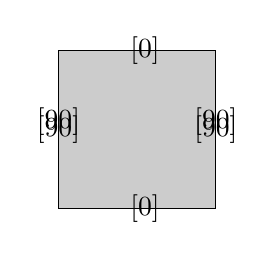
\begin{tikzpicture}[%
                scale=2,
                mypoint/.style={shape=circle, inner sep=1.5pt, color=black, fill}
            ]
            \draw [fill=black!20] 
                (0,0) -- (1,0) node [pos=0.55] {\myarrow[0]}
                      -- (1,1) node [pos=0.50] {\myarrow[90]}
                               node [pos=0.55] {\myarrow[90]}
                      -- (0,1) node [pos=0.45] {\myarrow[0]}
                      -- (0,0) node [pos=0.45] {\myarrow[90]}
                               node [pos=0.50] {\myarrow[90]};
        \end{tikzpicture}
    \end{center}
    Diese Beobachtung können wir nun benutzen, um eine Triangulierung des Torus
    zu konstruieren. Dabei müssen wir aber vorsichtig sein, denn zum Beispiel
    stellt 
    \begin{center}
        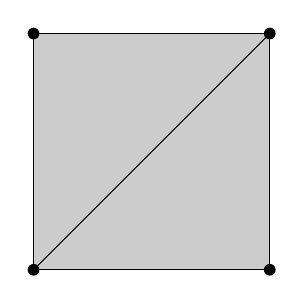
\begin{tikzpicture}[%
                scale=3,
                mypoint/.style={shape=circle, inner sep=1.5pt, color=black, fill}
            ]
            \draw [fill=black!20] (0,0) rectangle (1,1);
            \draw (0,0) -- (1,1);
            \foreach \mycoord in {(0,0),(0,1),(1,0),(1,1)}
                \node [mypoint] at \mycoord {};
        \end{tikzpicture}
    \end{center}
    eine gültige Triangulierung des Quadrats dar, wenn wir aber die Seiten wie
    zuvor miteinander identifizieren, so bilden die dargestellten Dreiecke
    keinen simplizialen Komplex mehr! (Warum?) Wir benötigen also eine feinere
    Triangulierung des Ausgangsquadrats, zum Beispiel folgende:
    \begin{center}
        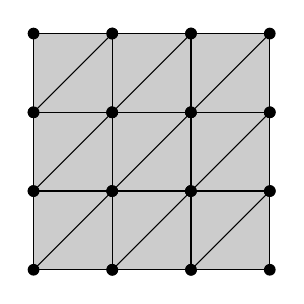
\begin{tikzpicture}[%
                mypoint/.style={shape=circle, inner sep=1.5pt, color=black, fill}
        ]
            \foreach \myx in {0,1,2} {
                \foreach \myy in {0,1,2} {
                    \begin{scope}[shift={(\myx,\myy)}]
                        \draw [fill=black!20] (0,0) rectangle (1,1);
                        \draw (0,0) -- (1,1);
                        \foreach \mycoord in {(0,0),(0,1),(1,0),(1,1)}
                        \node [mypoint] at \mycoord {};
                    \end{scope}
                }
            }
        \end{tikzpicture}
    \end{center}
    Identifizieren wir nun die äußeren Seiten, so sehen wir, dass wir eine
    Triangulierung des Torus gefunden haben.\footnote{%
        Es gibt Triangulierungen des Torus mit weniger $2$-Simplizes. Allerdings
        kann man zeigen, dass man mindestens $14$~Dreiecke benötigt, siehe
        z.\,B. Pelletier\cite{www:blog:rip:triangulation}.%
    }
    Im Allgemeinen müssen wir also genau aufpassen, ob eine gegebene
    Triangulierung nach Bildung eines Quotienten immer noch die Bedingungen
    eines simplizialen Komplexes erfüllt. 
\end{thBeispiel}

